\documentclass[10pt,letterpaper]{article}
\usepackage[top=1in,bottom=1in,left=1in,right=1in]{geometry}
\usepackage{datetime}
\usepackage{natbib}      % http://merkel.zoneo.net/Latex/natbib.php
\usepackage{palatino}
\usepackage{verbatim}
\usepackage[normalem]{ulem}
\bibpunct{(}{)}{;}{a}{,}{,}

\usepackage{array}

\usepackage{chngpage}
\usepackage{stmaryrd}
\usepackage{amssymb}
\usepackage{amsmath}
\usepackage{graphicx}
\usepackage{lscape}
\usepackage{subfigure}
\usepackage[usenames,dvipsnames]{color}
\definecolor{myblue}{rgb}{0,0.1,0.6}
\definecolor{mygreen}{rgb}{0,0.3,0.1}
\usepackage[colorlinks=true,linkcolor=black,citecolor=mygreen,urlcolor=myblue]{hyperref}

\newcommand{\bocomment}[1]{\textcolor{Bittersweet}{BO says: #1}}

\newcommand{\ignore}[1]{}
\newcommand{\transpose}{^\mathsf{T}}
\newcommand{\inner}[1]{\langle #1 \rangle} 
\newcommand{\smallsec}[1]{\noindent \textbf{#1\ }}
\newcommand{\cmd}[1] {{\color{blue}\texttt{#1}}}

\newcommand{\solution}[1]{{\color{myblue} \emph{[Solution:} 

#1 

\emph{End solution]}}}
\newcommand{\solutionnote}[1]{{\color{myblue} \emph{[Note:}

#1 

\emph{End note]}}}
\newcommand{\points}[1]{{\color{mygreen}\emph{[#1]\ \ }}}

\newcommand{\aone}{\diamondsuit}
\newcommand{\atwo}{\heartsuit}
\newcommand{\bone}{\triangle}
\newcommand{\btwo}{\Box}
\newcommand{\myand}{\ \land\ }
\newcommand{\myor}{\ \lor\ }
\newcommand{\mynot}{\lnot}

\title{
  \textbf{Mini-project 1: Color images} \\
  \Large{CMPSCI 670, Fall 2016, UMass Amherst} \\
  \Large{Due:  September 29, 1:00 PM } \\
  \Large{Instructor: Subhransu Maji} \\
  \Large{TA: Tsung-Yu Lin}
}

\settimeformat{ampmtime}
\date{}
\begin{document}
\maketitle

\renewcommand\thesubsection{\thesection.\alph{subsection}}


\section*{Guidelines}

\paragraph{Submission.} Submit a \emph{single pdf document} via moodle that includes your solutions, figures and printouts of code. For readability you may attach the code printouts at the end of the solutions. You could have 24 hours late submission with a 50\% mark down. Late submission beyond 24 hours will not be given \emph{any} credits. 

\paragraph{Plagiarism.} We might reuse problem set questions from previous years, covered by papers and webpages, we expect the students not to copy, refer to, or look at the solutions in preparing their answers. We expect students to want to learn and not google for answers. 

\paragraph{Collaboration.} The homework must be done individually, except where otherwise noted in the assignments. 'Individually' means each student must hand in their own answers, and each student must write their own code in the programming part of the assignment. It is acceptable, however, for students to collaborate in figuring out answers and helping each other solve the problems. We will be assuming that you will be taking the responsibility to make sure you personally understand the solution to any work arising from such a collaboration.

\paragraph{Using other programming languages.} All of the starter code is in Matlab which is what we expect you to use. You are free to use other languages such as Octave or Python with the caveat that we won't be able to answer or debug non Matlab questions.


\newpage
\section{Aligning Prokudin-Gorskii images [25 points]} 
Sergei Mikhailovich Prokudin-Gorskii (1863-1944) was a man well ahead of his time. Convinced, as early as 1907, that color photography was the wave of the future, he won Tzar's special permission to travel across the vast Russian Empire and take color photographs of everything he saw including the only color portrait of \href{https://en.wikipedia.org/wiki/Leo_Tolstoy}{Leo Tolstoy}. And he really photographed everything: people, buildings, landscapes, railroads, bridges... thousands of color pictures! His idea was simple: record three exposures of every scene onto a glass plate using a red, a green, and a blue filter. Never mind that there was no way to print color photographs until much later -- he envisioned special projectors to be installed in "multimedia" classrooms all across Russia where the children would be able to learn about their vast country. Alas, his plans never materialized: he left Russia in 1918, right after the revolution, never to return again. Luckily, his RGB glass plate negatives, capturing the last years of the Russian Empire, survived and were purchased in 1948 by the Library of Congress. The LoC has recently digitized the negatives and made them available on-line.\footnote{This description and assignment is courtesy Alyosha Efros @ UC Berkeley }
\begin{figure}[h]
\centering
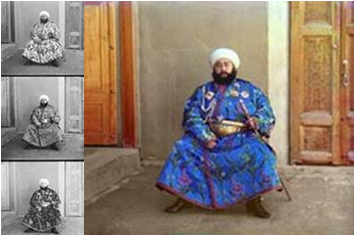
\includegraphics[width=0.65\linewidth]{example-Prokudin-Gorskii.png}
\caption{Example image from the Prokudin-Gorskii collection. On the left are the three images captured individually. On the right is a reconstructed color photograph. Note the colors are in B, G, R order from the top to bottom (and not R, G, B)!}
\end{figure}

Your goal is to take photographs of each plate and generate a color image by aligning them (Figure 1). The easiest way to align the plates is to exhaustively search over a window of possible displacements (say [-15,15] pixels), score each one using some image matching metric, and take the displacement with the best score. There is a number of possible metrics that one could use to score how well the images match. The simplest one is just the L2 norm also known as the Sum of Squared Differences (SSD) distance which is simply \cmd{sum(sum((image1-image2)$.^\wedge$2))} where the sum is taken over the pixel values. Another is normalized cross-correlation (NCC), which is simply a dot product between two normalized vectors: \cmd{(image1./||image1||} and \cmd{image2./||image2||)}. Note that in the case of the Emir of Bukhara (Figure 1), the images to be matched do not actually have the same brightness values (they are different color channels), so you might have to use a cleverer metric, or different features than the raw pixels.

\subsection{Code}
Download the \cmd{p1\_code.tar.gz} and \cmd{p1\_data.tar.gz} from the moodle page. The latex sources are also available as \cmd{p1\_latex.tar.gz}. Move them to your homework directory and extract the files (e.g. by typing \cmd{tar -xvf p1\_code.tar.gz}). 

Before you start aligning the Prokudin-Gorskii images (in $\cmd{data/prokudin-gorskii}$), you will test your code on synthetic images which have been randomly shifted. Your code should correctly discover the inverse of the shift.

Run \cmd{evalAlignment.m} on the Matlab command prompt inside the code directory. This should produce the following output. Note the actual 'gt shift' might be different since it is randomly generated.
\begin{verbatim}
    Evaluating alignment ..
    1 balloon.jpeg
	   gt shift: ( 1,11) ( 4, 5)
	 pred shift: ( 0, 0) ( 0, 0)
    2 cat.jpg
	   gt shift: (-5, 5) (-6,-2)
	 pred shift: ( 0, 0) ( 0, 0)
     ...
\end{verbatim}
    
The code loads a set of images, randomly shifts the color channels and provides them as input to \cmd{alignChannels.m}. Your goal is to implement this function. A correct implementation should obtain the shifts that is the negative of the ground-truth shifts, i.e. the following output:

\begin{verbatim}
    Evaluating alignment ..
    1 balloon.jpeg
	   gt shift: ( 13, 11)  ( 4, 5)
	 pred shift: (-13,-11)  (-4,-5)
    2 cat.jpg
	   gt shift: (-5, 5) (-6,-2)
	 pred shift: ( 5,-5) ( 6, 2)
     ...
\end{verbatim}
    
Once you are done with that, run \cmd{alignProkudin.m}. This will call your function to align images from the Prokudin-Gorskii collection. The output is saved to the \cmd{outDir}. Note: if this directory already exists then the results will be overwritten.


\subsection{What to submit?}
To get full credit for this part you have to 
\begin{itemize}
\item include your implementation of \cmd{alignChannels.m},
\item verify that the \cmd{evalAlignment.m} correctly recovers the color image and shifts for the toy example and include the output results.
\item include the aligned color images from the output of \cmd{alignProkudin.m},
\emph{including} the computed shift vectors for each image.
\end{itemize}

\subsection{Some tips}
\begin{itemize}
\item Look at functions \cmd{circshift()} and \cmd{padarray()} to deal with shifting images.

\item How to include code in latex? Answer: The ``verbatim" package provides ways to include pasted code, or code from a file, in its raw format. For example you can include the code in a file \cmd{alignChannels.m} by typing: 
\begin{verbatim}
\verbatiminput{../solution/alignChannels.m}}.
\end{verbatim}

\item Shifting images can cause ugly boundary artifacts. You might find it useful to crop the image after the alignment.
\end{itemize}



\newpage
\section{Color image demosaicing [30 points]}
Recall that in digital cameras the red, blue, and green sensors are interlaced in the Bayer pattern (Figure~\ref{fig:bayer}). The missing values are interpolated to obtain a full color image. In this part you will implement several interpolation algorithms. The input to the algorithm is a single image im, a NxM array of numbers between 0 and 1. These are measurements in the format shown in Figure~\ref{fig:bayer}, i.e., top left \cmd{im(1,1)} is red, \cmd{im(1,2)} is green, \cmd{im(2,1)} is green, \cmd{im(2,2)} is blue, etc. Your goal is to create a single color image C from these measurements.
\begin{figure}[h]
\centering
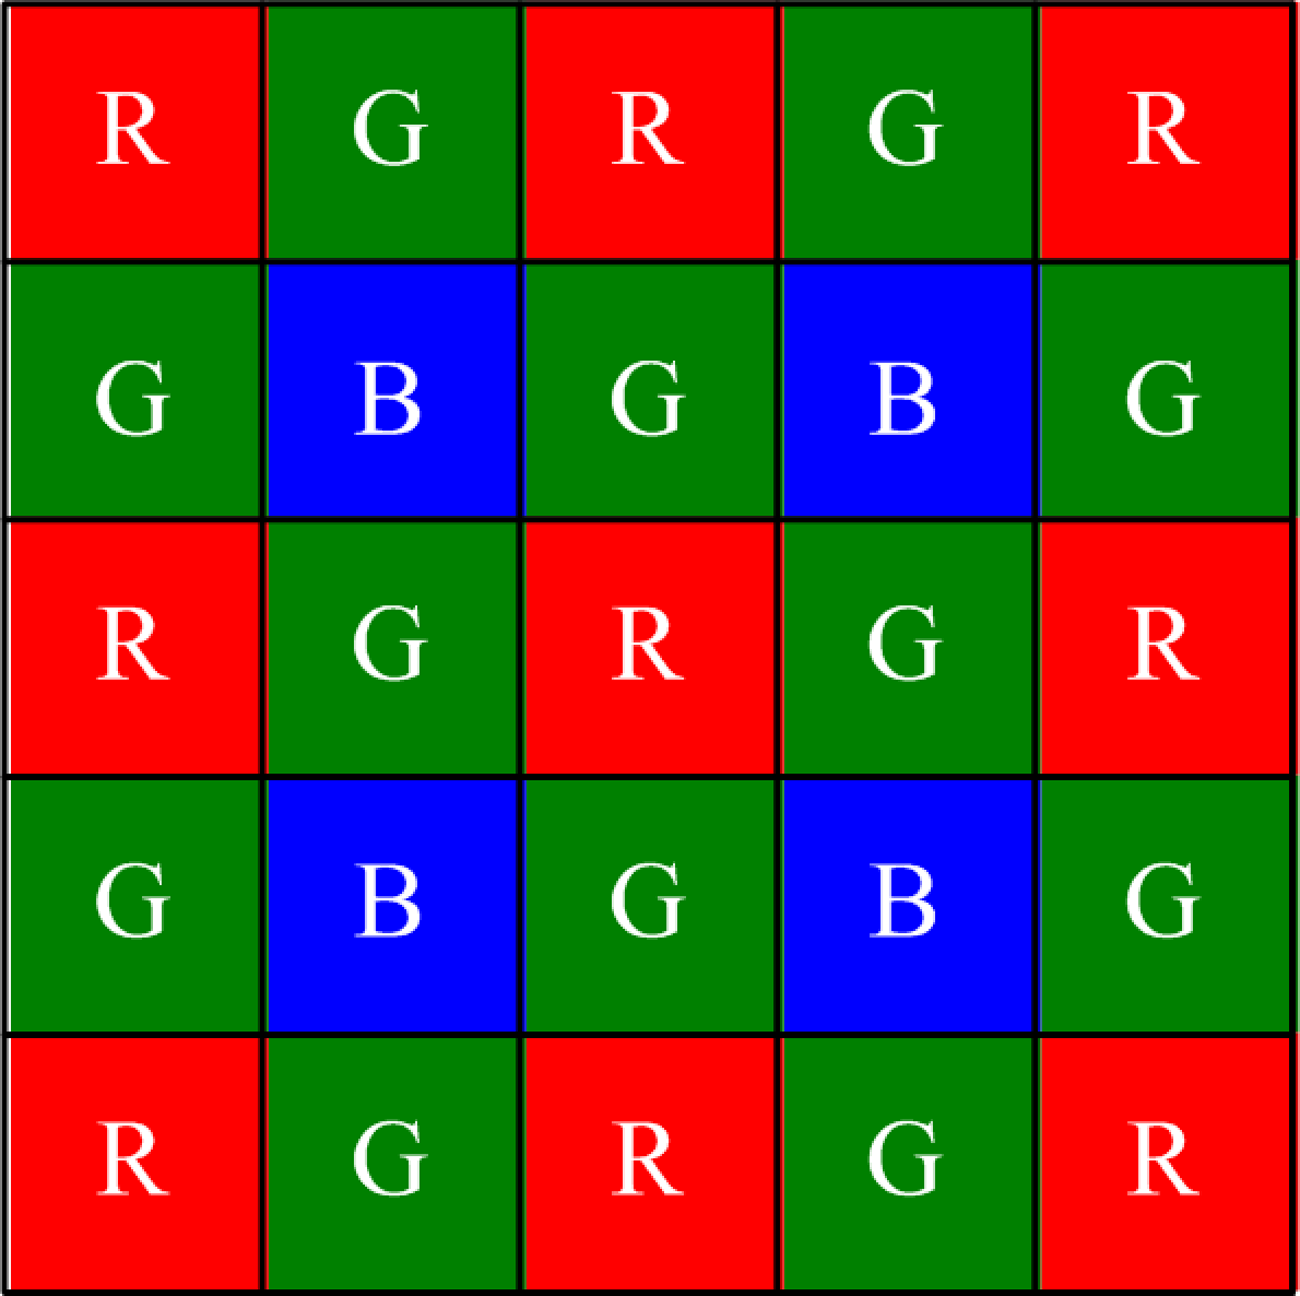
\includegraphics[width=0.2\linewidth]{bayer-pattern.png}
\caption{\label{fig:bayer} Bayer pattern}
\end{figure}

\subsection{Code}
Your entry point for this part of the homework is in \cmd{evalDemosaic.m}. The code loads images from the data directory (in $\cmd{data/demosaic}$), artificially mosaics them (\cmd{mosaicImage.m} file), and provides them as input to the demosaicing algorithm (\cmd{demosaicImage.m} file). By comparing the result with the input we can also compute the reconstruction error measured as the distance between the reconstructed image and the true image. This is what the algorithm reports. Once you have implemented the \cmd{mosaicImage} function run the \cmd{evalDemosaic.m} and you should see the output below.

Right now only the \cmd{demosaicImage(im, 'baseline')} is implemented which simply replaces all the missing values for a channel with the average value of that channel. All the other methods call the baseline algorithm hence they produce identical results. Implement the following functions in the file:

\begin{itemize}
\item \points{10 points} \cmd{demosaicImage(im, 'nn')} -- nearest-neighbour interpolation.
\item \points{10 points} \cmd{demosaicImage(im, 'linear')} -- linear interpolation.
\item \points{10 points} \cmd{demosaicImage(im, 'adagrad')} -- adaptive gradient interpolation.
\end{itemize}

In class we discussed how to interpolate the green channel. For the red and blue channels the algorithms will be different since there are half as many pixels with sampled values. For the adaptive gradient method start by interpolating only the green channel and using linear interpolation for the other two channels. Once the overall performance is better, think of a way of improving the interpolation for the red and blue channels. You can even apply different strategies to different pixels for the same channel! 

For reference, the baseline method achieves an average error of 0.1392 across the 10 images in the dataset. Your methods you should be able to achieve substantially better results. The linear interpolation method achieves an error of about 0.017. You should report the results of all your methods in the form of the table below.

\newpage

\begin{verbatim}
----------------------------------------------------------------------------
# 	 image             baseline      nn       linear     adagrad
----------------------------------------------------------------------------
1 	 balloon.jpeg      0.179239 	 0.179239 	 0.179239 	 0.179239 
2 	 cat.jpg           0.099966 	 0.099966 	 0.099966 	 0.099966 
3 	 ip.jpg            0.231587 	 0.231587 	 0.231587 	 0.231587 
4 	 puppy.jpg         0.094093 	 0.231587 	 0.231587 	 0.231587 
5 	 squirrel.jpg      0.121964 	 0.231587 	 0.231587 	 0.231587 
6 	 pencils.jpg       0.183101 	 0.183101 	 0.183101 	 0.183101 
7 	 house.png         0.117667 	 0.117667   0.117667   0.117667 
8 	 light.png         0.097868 	 0.097868 	 0.097868 	 0.097868 
9 	 sails.png         0.074946 	 0.074946 	 0.074946 	 0.074946 
10  tree.jpeg         0.167812 	 0.167812 	 0.167812 	 0.167812 
----------------------------------------------------------------------------
 	 	average 	        	0.136824 	 0.136824 	 0.136824 	 0.136824 
----------------------------------------------------------------------------
\end{verbatim}

Tips: You can visualize at the errors by setting the display flag to true in the \cmd{runDemosaicing.m}. Avoid loops for speed in MATLAB. Be careful in handling the boundary of the images. It might help to think of various operations as convolutions. Look up MATLAB's conv2() function that implements 2D convolutions.

\subsection{What to submit?}
To get full credit for this part you have to 
\begin{itemize}
\item include your implementation of \cmd{demosaicImage.m}, 
\item include the output of \cmd{evalDemosaic.m},
\item clearly describe the implementation details.
\end{itemize}

\newpage
\section{Extensions [10 points]}
Implement at least one of the following to get up to 10 points. You can implement multiple for extra credit!

\begin{itemize}
\item \textbf{Transformed color spaces for demosaicing.} Try your demosaicing algorithms by first interpolating the green channel and then transforming the red and blue channels R $\leftarrow$ R/G and B $\leftarrow$ B/G, i.e., dividing by the green channel and then transforming them back after interpolation. Try other transformations such as logarithm of the ratio, etc (note: you have to apply the appropriate inverse transform). Does this result in better images measured in terms of the mean error? Why is this a good/bad idea? 

\item \textbf{Coarse-to-fine alignment.} Searching over displacements can be slow. Think of a way of aligning them faster in a coarse-to-fine manner. For example you may align the channels by resizing them to half the size and then refining the estimate. This can be done by multiple calls to your alignChannels() function. If you implement this part then you can try your method on the high resolution .tif images in the \url{http://inst.eecs.berkeley.edu/~cs194-26/fa16/hw/proj1/data/} directory.

\item \textbf{Evaluate alternative sampling patterns.} Come up with a way of finding the optimal 2x2 pattern for color sampling. You can further simplify this problem by fixing the interpolation algorithm to linear and only using non-panchromatic cells (i.e, no white cells). A brute-force approach is to simply enumerate all the $3^4 = 81$ possible patterns and evaluate the error on a set of images and pick the best. What patterns work well? What are their properties (e.g., ratio of red, blue, green, cells)?

\end{itemize}
\end{document}
